\section{Image data formats}
As everything else, images are encoded as a sequence of bits.
How we structure these bits in memory is another important property of image formats and can be very important for performance.
Normal RGB images are encoded as three 8-bit values for each pixel, one for each color channel.


\subsection{Interleved vs planar vs semi-planar}
There are three main ways to store the color channels in memory, interleved, planar and semi-planar \cite{baranYUVFormats2018}.
In interleved formats, the color channels are stored in sequence, i.e. RGBRGBRGB.
In planar formats, the color channels are stored in separate arrays, i.e. RRRBBBGGG.
Semi-planar formats are a mix of the two where some channels are interleved and some are planar, i.e. RRRGBGBGB.
The reson one might be preferred over the other is to optimize for memory locality.
For instance, if you are performing per-bit operations, having the bits of the same color channel next to each other is beneficial.


\begin{figure}[H]
    \centering
    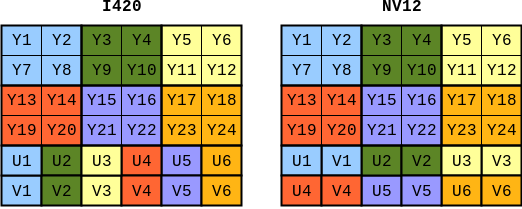
\includegraphics[width=.8\textwidth]{figures/debayer/YUV_packaging.png}
    \caption{Visualization of I420 and NV12, two popular YUV 4:2:0 formats \cite{baranYUVFormats2018}.}
    \label{fig:image_packaging}
\end{figure}

\subsection{Bit depth and packaging}
A final importnt property of image formats is the bit depth, i.e. how many bits are used to represent each pixel.
Most images use a single byte (8 bits) for each color channel, but higher bit depths offer better color fidelity and dynamic range.
How these bits are packaged might also vary.
If the number of bits is not divisable by 8, like for 10-bit images, the most space efficient way to store and send them is to pack them into 8-bit bytes, i.e. 4 10-bit values are stored in 5 bytes.
However as most \glspl{alu} do not support 10-bit operations, padding the to the neares full byte is better for computations.

